
\documentclass[11pt,oneside,a4wide]{report}

\usepackage[ngerman]{babel}
\usepackage{graphicx}
\usepackage[svgnames,table,hyperref]{xcolor}
\usepackage{amssymb}
\usepackage{mathtools}
\usepackage{setspace}
\usepackage{listings}
%\usepackage[hyperindex,hidelinks]{hyperref}
\usepackage[hyperindex]{hyperref}

\onehalfspacing

\lstdefinestyle{customXML}{
    belowcaptionskip=1\baselineskip,
    breaklines=true,
    frame=L,
    xleftmargin=\parindent,
    language=XML,
    showstringspaces=false,
    basicstyle=\footnotesize\ttfamily,
    keywordstyle=\bfseries\color{green!40!black},
    commentstyle=\itshape\color{purple!40!black},
    identifierstyle=\color{blue},
    stringstyle=\color{orange},
    numbers=left,
    numberstyle=\tiny,
}
\lstdefinestyle{customSQL}{
    belowcaptionskip=1\baselineskip,
    breaklines=true,
    frame=L,
    xleftmargin=\parindent,
    language=SQL,
    showstringspaces=false,
    basicstyle=\footnotesize\ttfamily,
    keywordstyle=\bfseries\color{green!40!black},
    commentstyle=\itshape\color{purple!40!black},
    identifierstyle=\color{blue},
    stringstyle=\color{orange},
    numbers=left,
    numberstyle=\tiny,
}
\lstdefinestyle{customHTML}{
    belowcaptionskip=1\baselineskip,
    breaklines=true,
    frame=L,
    xleftmargin=\parindent,
    language=HTML,
    showstringspaces=false,
    basicstyle=\footnotesize\ttfamily,
    keywordstyle=\bfseries\color{green!40!black},
    commentstyle=\itshape\color{purple!40!black},
    identifierstyle=\color{blue},
    stringstyle=\color{orange},
    numbers=left,
    numberstyle=\tiny,
}

\newcommand{\HRule}{\rule{\linewidth}{0.5mm}}

\begin{document}

\begin{titlepage}
    \begin{center}

    % Title
    \HRule \\[0.4cm]
    { \huge \bfseries PIM L"osungen\\"Ubung\\[0.4cm] }
    \HRule \\[1.5cm]

    \textbf{Achtung: Dies ist keine offizielle L"osung!}

    \vfill
    Von:\\
    Dustin Wind


   \vfill
    Zuletzt modifiziert am:\\
    {\large \today}\\
    \end{center}
    \bigskip

    {\small
    Bentuzte Software:
    \begin{itemize}
        \item \href{http://www.latex-project.org}{\LaTeX{}: structured text formatting and typesetting}
        \item \href{https://wiki.gnome.org/Apps/Dia/}{Dia: a diagram drawing program}
    \end{itemize}
    }

\end{titlepage}

%\maketitle

\tableofcontents

%\include{inc/Test/test}


\chapter{Aufgabenblatt 01}
\section{Lastenheft}
Da auch die Hochschule mit der Zeit gehen und ihre Studenten bestm¨oglich infomrieren will hat der Dekan beschlossen, eine mobile Applikation entwickeln zu lassen.
Als erstes Modul soll ein Mensa-Informations-System erstellt werden.
Umd die Anwendung in das Budget der Universit¨at einplanen zu k"onnen, bittet man Ihre Abteilung um ein Angebot.\\

\noindent
Sie arbeiten als Software Architekt in der IT-Abteilung der Universit¨at.
Ihr Chef bittet Sie, das vom Dekan erstellte Dokument in ein Anforderungsdokument zu "uberf"uhren.

\subsection{Aufgabe 1: Anforderungsanalyse}
Analysieren Sie das Dokument und "uberlegen Sie sich, ob es m"oglich ist, auf Basis dieser Beschreibung ein Angebot zu erstellen:
\begin{enumerate}
    \item Die Anwendung soll einfach und intuitiv zu bedienen sein und der Gro"steil der Studenten soll sie nutzen k"onnen
    \item Es ist wichtig, dass die Software ansprechend gestaltet ist und den Studenten das Leben vereinfacht
    \item Die App soll die jeweiligen Mensa-Standorte anzeigen k"onnen
    \item Es soll m"oglich sein, die Gerichte der Mensa zu bewerten
    \item Es soll m"oglich sein, wichtige Informationen zur Mensa anzeigen zu lassen
\end{enumerate}

\textbf{L"osung:}
\begin {enumerate}
    \item Die Begriffe "`einfach"',"´intuitiv"',"´Gro"steil"' sind nicht genau spezifiziert, somit nicht SMART- konform
    \item Die Begriffe "´ansprechend gestaltet"' und "´das Leben vereinfacht"' sind nicht genau spezifiziert
    \item Diese Anforderung passt so, wie sie ist
    \item Diese Anforderung passt ebenfalls
    \item Der Begriff "´wichtige Informationen"' sollte n"aher spezifiziert sein
\end{enumerate}
    
\subsection{Aufgabe 2: Erstellung Anforderungsdokument}
Um den Dekan bestm"oglich zu unterst"utzen, erstellen Sie einen Vorschlag f"ur ein detailliertes Anforderungsdokument, das als Grundlage f"ur die sp"atere Entwicklung dienen soll. 
Bitte nutzen Sie dazu die vom Dekan gemachten Angaben als Basis.

\textbf{L"osung:}
\begin{enumerate}
    \item Die app soll eine Einstiegsseite mit einem "Uberblick "uber die Funktionen der App bieten 
    \item Es soll eine Karte mit den relevanten Mensa- Standorten eingebunden werden, welche eine Navigationsm"oglichkeit enth"alt 
    \item Es soll ein Mensa- Modul enthalten sein, welches den Speiseplan und Bewertungsfunktionen enth"alt 
    \item Eine Anbindung an das UNIVIS soll vorhanden sein 
    \item Es soll m"oglich sein, den eigenen Vorlesungsplan zu hinterlegen
    \item E- Learning- Inhalte sollen integriert sein 
    \item "Uber eine Facebook- Anbindung sollen Community-Features inkl. Diskussionsforum realisiert werden 
    \item Das Projekt soll durch Werbung finanziert werden 
    \item Eine Anzeige von Veranstaltungen des t"aglichen Studentenlebens soll m"oglich sein
\end{enumerate}




\chapter{Aufgabenblatt 02}

\section{HTML}
Sie sind weiterhin mit der Erstellung des Mensa Moduls f"ur die mobile Anwendung der Universit"at beauftragt.
Mittlerweise wurde entschieden, die Anwendung in Form einer mobilen Webseite zu implementieren.
Um sich mit HTML vertraut zu machen versuche Sie, die folgende Struktur als HTML Seite umzusetzen.

\subsection{Erstellung eines HTML-Dockuments}
Erstellen Sie ein neues HTML Dokument mit dem nahem "`MensaApp.html"':
\begin{itemize}
    \item Seitentitel: "`MensaApp"'
    \item "Uberschrift $h1$: "`MensaApp der FAU""
    \item Einf"uhrender Text: "`Herzlich Willkommen auf der Startseite"' in fetter Schrift
    \item Freitext in neuem Absatz: "`Als Student haben Sie die M"oglichkeit an folgenden Mensen zu speisen:"'
    \item Ungeordnete Liste mit folgenden Eintr"agen:
    \begin{itemize}
        \item Mensa Langemarckplatz
        \item S"udmensa
        \item Mensa Insel Sch"utt
        \item Mensa Regensburger Stra"se
        \item Ausgabemensa St. Paul
        \item Mensateria Ohm
    \end{itemize}
    \item Die einzelnen Eintr"age sollen auf die jeweiligen Links zu den entsprechenden Speisepl"anen verweisen, welche hier zu finden sind: \url{http://www.studentenwerk.uni-erlangen.de/verpflegung/de/speiseplaene.shtml}
    \item Pr"ufen Sie das HTML Dokument, indem Sie es sich im Browser anzeigen lassen
\end{itemize}

\lstset{style=customHTML}
\lstinputlisting[style=customHTML]{./inc/aufgabe02/mensaapp.html}



\chapter{Aufgabenblatt 03}


\section{Datenmodellierung}

\subsection{Aufgabe 1: ERM}

Ihnen liegt der nachfolgende Auszug aus dem Pflichtenheft vor. Bitte "uberf"uhren Sie diesen in ein Entity-Relationship-Diagramm mit Chen Notation.
Bestimmen Sie dazu die relevanten Entity-Typen, deren Beziehung untereinander soweie deren Kardinalit"aten und Attribute.
Bestimmen Sie daraufhin die jeweiligen Schl"usselattribute.\\

\textbf{Auszug aus dem Pflichtenheft}
\begin{itemize}
    \item Jede Mensa ist eindeutig durch einen Namen, Ort und eine Dienststellennummer charakterisiert und wird durch einen Mensa-Chef geleitet.
    Dieser besitzt neben seinem Namen und Vornamen auch eine Personalnummer und einen Rang.
    Es kann auch m"oglich sein, dass der Chef f"ur mehr als eine Mensa Zust"andig ist.
    \item Jede Mensa bietet verschiedene Gerichte an.
    Es handelt sich dabei entweder um dauerhafte Angebote oder ein saisonales "`Special"'.
    Um die Zuordnung zu vereinfachen besitzt jedes der Gerichte eine interne Referenznummer, einen Namen und eine Beschreibung.
    Es kann sich dabei sowohl um eine Vor-, Haupt-, oder Nachspeise handeln.
    Die Gerichte haben dar"uber hinaus eine Bewertung, welche die Beliebtheit bei den Studenten widerspiegeln soll.
    Mede Mensa bietet zu unterschiedlichen Zeitpunkten unterschiedliche Gerichte an.
    \item Jedes der Gerichte besteht aus einer oder mehreren Zutaten.
    Diesen sind durch eine Bestelnummer und die Bezeichnung gekennzeichnet.
    Dar"uber hinaus dienen der Haltbarkeitszeitraum, die Angabe der m"oglichen Allergika sowie die Angabe ob vegetarisch oder nicht als wichtige Informationen.
\end{itemize}

\bigskip
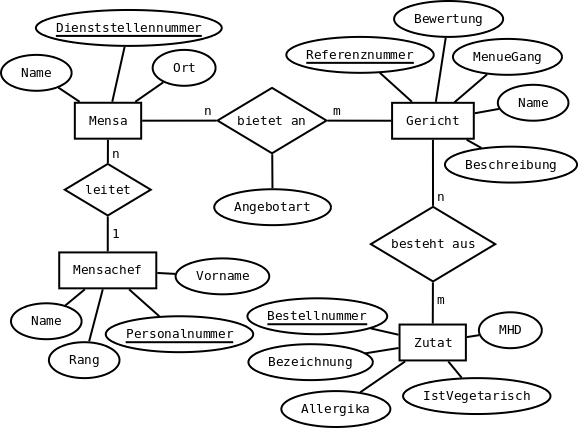
\includegraphics[scale=0.5]{./inc/aufgabe03/mensaapp.png}

\subsection{Aufgabe 2: Relationenschema}
"Uberf"uhren Sie nun das von Ihnen erstelte ERM-Diagramm in das Relationenmodell.\\

\noindent
\fbox{
    \parbox{\textwidth}{
        \textbf{Mensachef}(\underline{Personalnummer}, Name, Vorname, Rang)\\
        \textbf{Mensa}(\underline{Dienststellennummer, Name, Ort}, $\overline{Personalnummer}$)\\
        \textbf{Gericht}(\underline{Referenznummer}, Name, Beschreibung, Angebotart, MenueGang, Bewertung, $\overline{Mensa}$)\\
        \textbf{Zutat}(\underline{Bestellnummer}, Bezeichnung, MHD, Allergika, IstVegetarisch)\\
        \textbf{Rezept}(\underline{GerichtId[Gericht], ZutatId[Zutat]})\\
        
        \noindent
        {\small \textbf{Anm. des Autors}: Fremdschl"usselbeziehungen k"onnen entweder durch einen Oberstrich gekennzeichnet werden, oder durch das Angeben der Tabelle, auf die der  Fremdschl"ussel refenziert, in eckigen Klammern.\\
        Im Zweifel sollte w"ahrend der Klausur die Methode der Vorlesung gew"ahlt werden!}
    }
}




















\chapter{Aufgabenblatt 04}

\section{Datengest"utzte Anwendungen}
In der vergangenen Woche haben Sie das Relationenmodell f"ur die mobile Uni-Applikation erstellt.
Dies liegt mittlerweile in der Datenbank vor.
F"ur die Entwicklung des Mensa-Moduls ben"otigen Sie Ausschnitte aus dieser Datenbank f"ur die Anzeige auf dem mobilen Client.\\
In der Vorlesung haben Sie die Elemente von SQL-Abfragen kennen gelernt.


\subsection{Aufgabe 1: SQL}
Erstellen Sie eine Abgrage, die den Namen und die Bewertung aller Gerichte ausgibt, die in der Zentralmensa in N"urnberg angeboten werden.

\lstset{style=customSQL}
\begin{lstlisting}
SELECT      g.Name, g.Bewertung
FROM        Gericht AS g
            JOIN Speiseplan AS s ON g.Referenznummer = s.GerichtId
            JOIN Mensa AS m ON s.MensaId = m.Dienststellennummer
WHERE       m.Ort = 'Nuernberg'
            AND m.Name LIKE '%Zentralmensa%'
;
\end{lstlisting}

\subsection{Aufgabe 2: SQL}
Listen Sie den Namen und die Beschreibung aller vegetarischen Gerichte auf, die in den Mensen des Studentenwerks angeboten werden.
Beachten Sie dabei, dass ein Gericht nur dann vegetarisch ist, wenn alle Zutaten vegetarisch sind.\\

\lstset{style=customSQL}
\begin{lstlisting}
SELECT      Name, Beschreibung
FROM        Gericht
WHERE       Gericht.RefNum NOT IN
            (
                -- create a table with all meals containing meat
                SELECT      r.GerichtID
                FROM        Rezept AS r
                            LEFT OUTER JOIN 
                            (
                                SELECT  z.BestNum
                                FROM    Zutat AS z
                                WHERE   z.IstVegetarisch = 1
                            ) AS x
                            ON r.ZutatId = x.BestNum
                -- due to the left-outer join all 
                -- meat-containing meals in table r join x
                -- have their column 'BestNum' set to NULL
                WHERE       x.BestNum IS NULL
            )
;
\end{lstlisting}



\noindent
Beispiel-Tabelle (Rezept):\\
\rowcolors{1}{LightGrey}{White}
\begin{tabular}{ l l }
    \rowcolor{LightSlateGray}
    \textbf{GerichtId}  & \textbf{ZutatId}\\
    id(Currywurst)      & id(Wurst)\\
    id(Currywurst)      & id(Curry)\\
    id(Kartoffelpuffer) & id(Kartoffeln)\\
    id(Kartoffelpuffer) & id(Apfelmus)\\
\end{tabular}





\end{document}



